\subsection{Boltzmann Map Validation (ex 5)}

The numerical pipeline for primordial-to-late-time transfer mapping was validated using CLASS \parencite{Lesgourgues_2011} and CAMB \parencite{Lewis_2000} under matching cosmological parameters ($\Omega_{b,0} = 0.0493$, $\Omega_{cdm,0} = 0.2657$, $h = 0.6737$, $A_s = 2.1 \times 10^{-9}$, $n_s = 0.9649$) in Newtonian gauge at $z = 0$.

\subsubsection{Matter Spectrum Reconstruction and Unit Validation}

The linear matter power spectrum $P_m^{\mathrm{rec}}(k, z)$ was reconstructed directly from the primordial curvature power spectrum $P_{\mathcal{R}}(k)$ and the matter transfer function $T_m(k, z)$ via Eq~\ref{eq:matter_spectrum_reconstruction}. 
Figure~\ref{fig:pm_reconstruction} compares the reconstructed spectrum $P_m^{\mathrm{rec}}(k)$ against the direct CLASS output $P_m(k)$.

\begin{figure}[htbp]
    \centering
    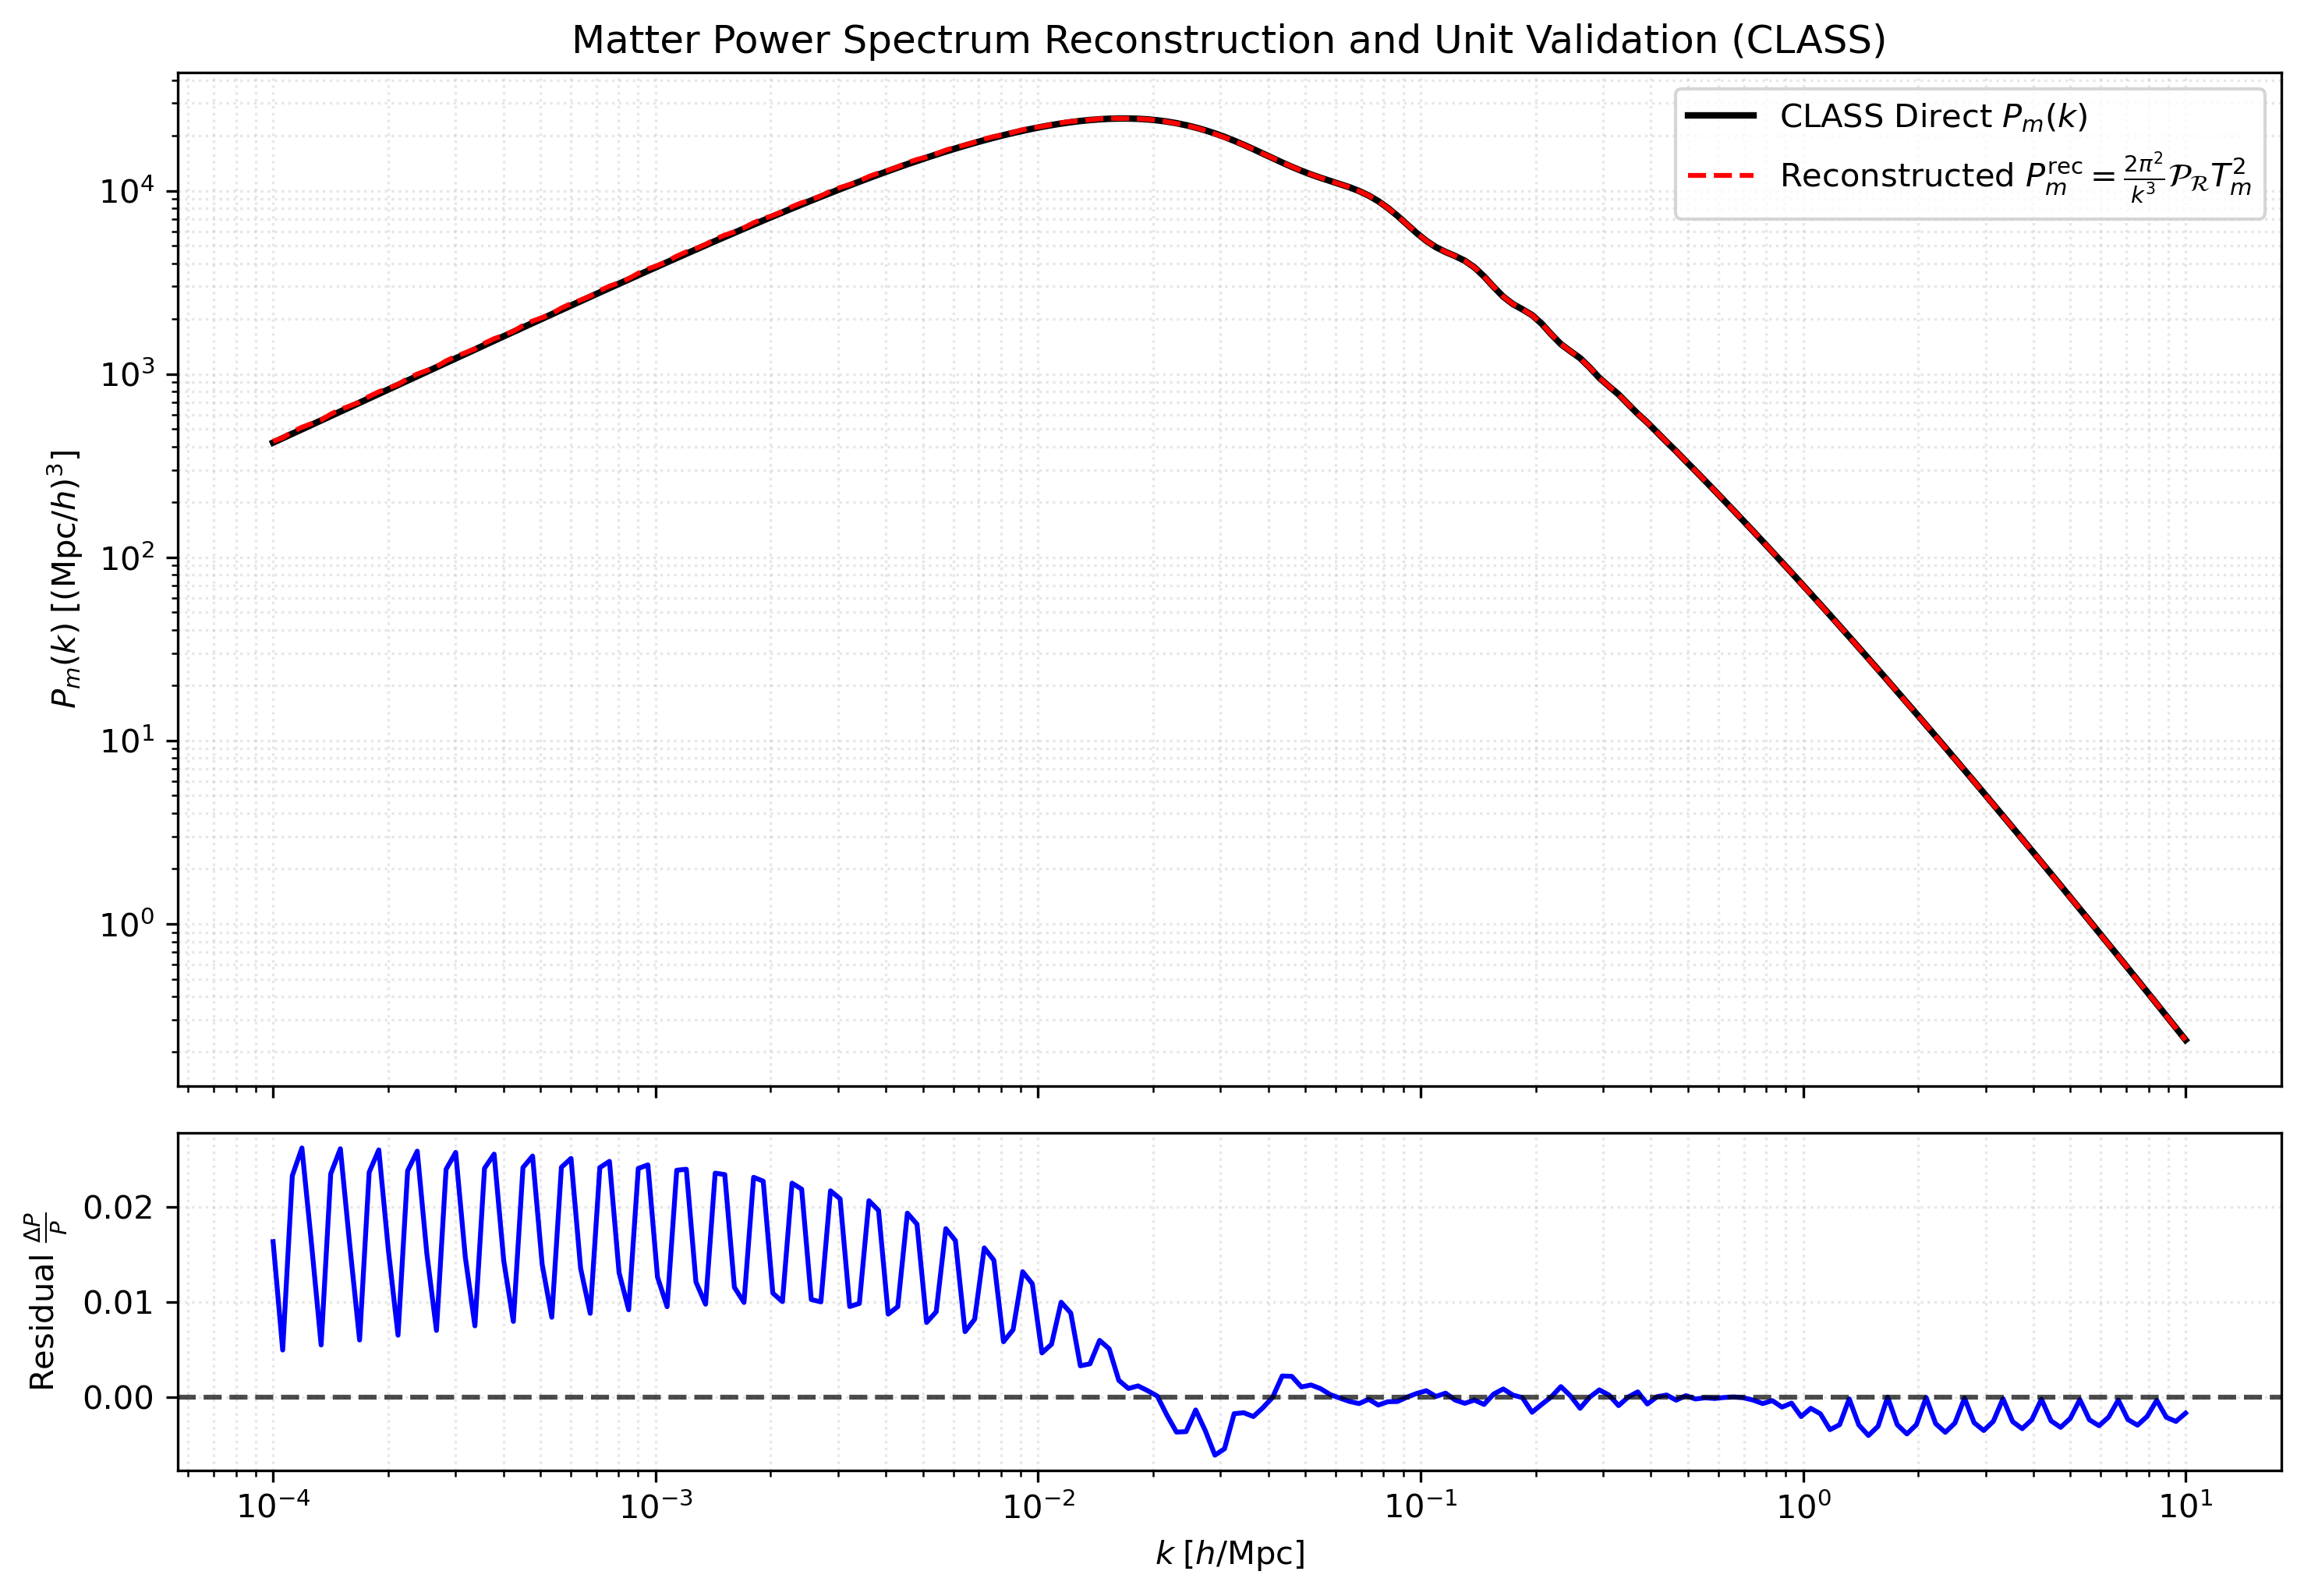
\includegraphics[width=0.82\textwidth]{New_Figures/Test_20261106_190746_Pm_reconstruction.png}
    \caption{Matter power spectrum reconstruction $P_m^{\mathrm{rec}}(k)$ compared against direct CLASS output $P_m(k)$ at $z=0$, validating unit conversions ($h\,\mathrm{Mpc}^{-1} \to \mathrm{Mpc}^{-1}$ and $(\mathrm{Mpc}/h)^3 \to \mathrm{Mpc}^3$) and transfer normalization.}
    \label{fig:pm_reconstruction}
\end{figure}

\subsubsection{Numerical Precision and Convergence Test}

To isolate numerical solver integration controls from physical modeling, CLASS was executed with tightened precision settings (rtol = $10^{-8}$, atol = $10^{-10}$, $k_\text{per decade}$ = 100).
    \begin{figure}[htbp]
        \centering
        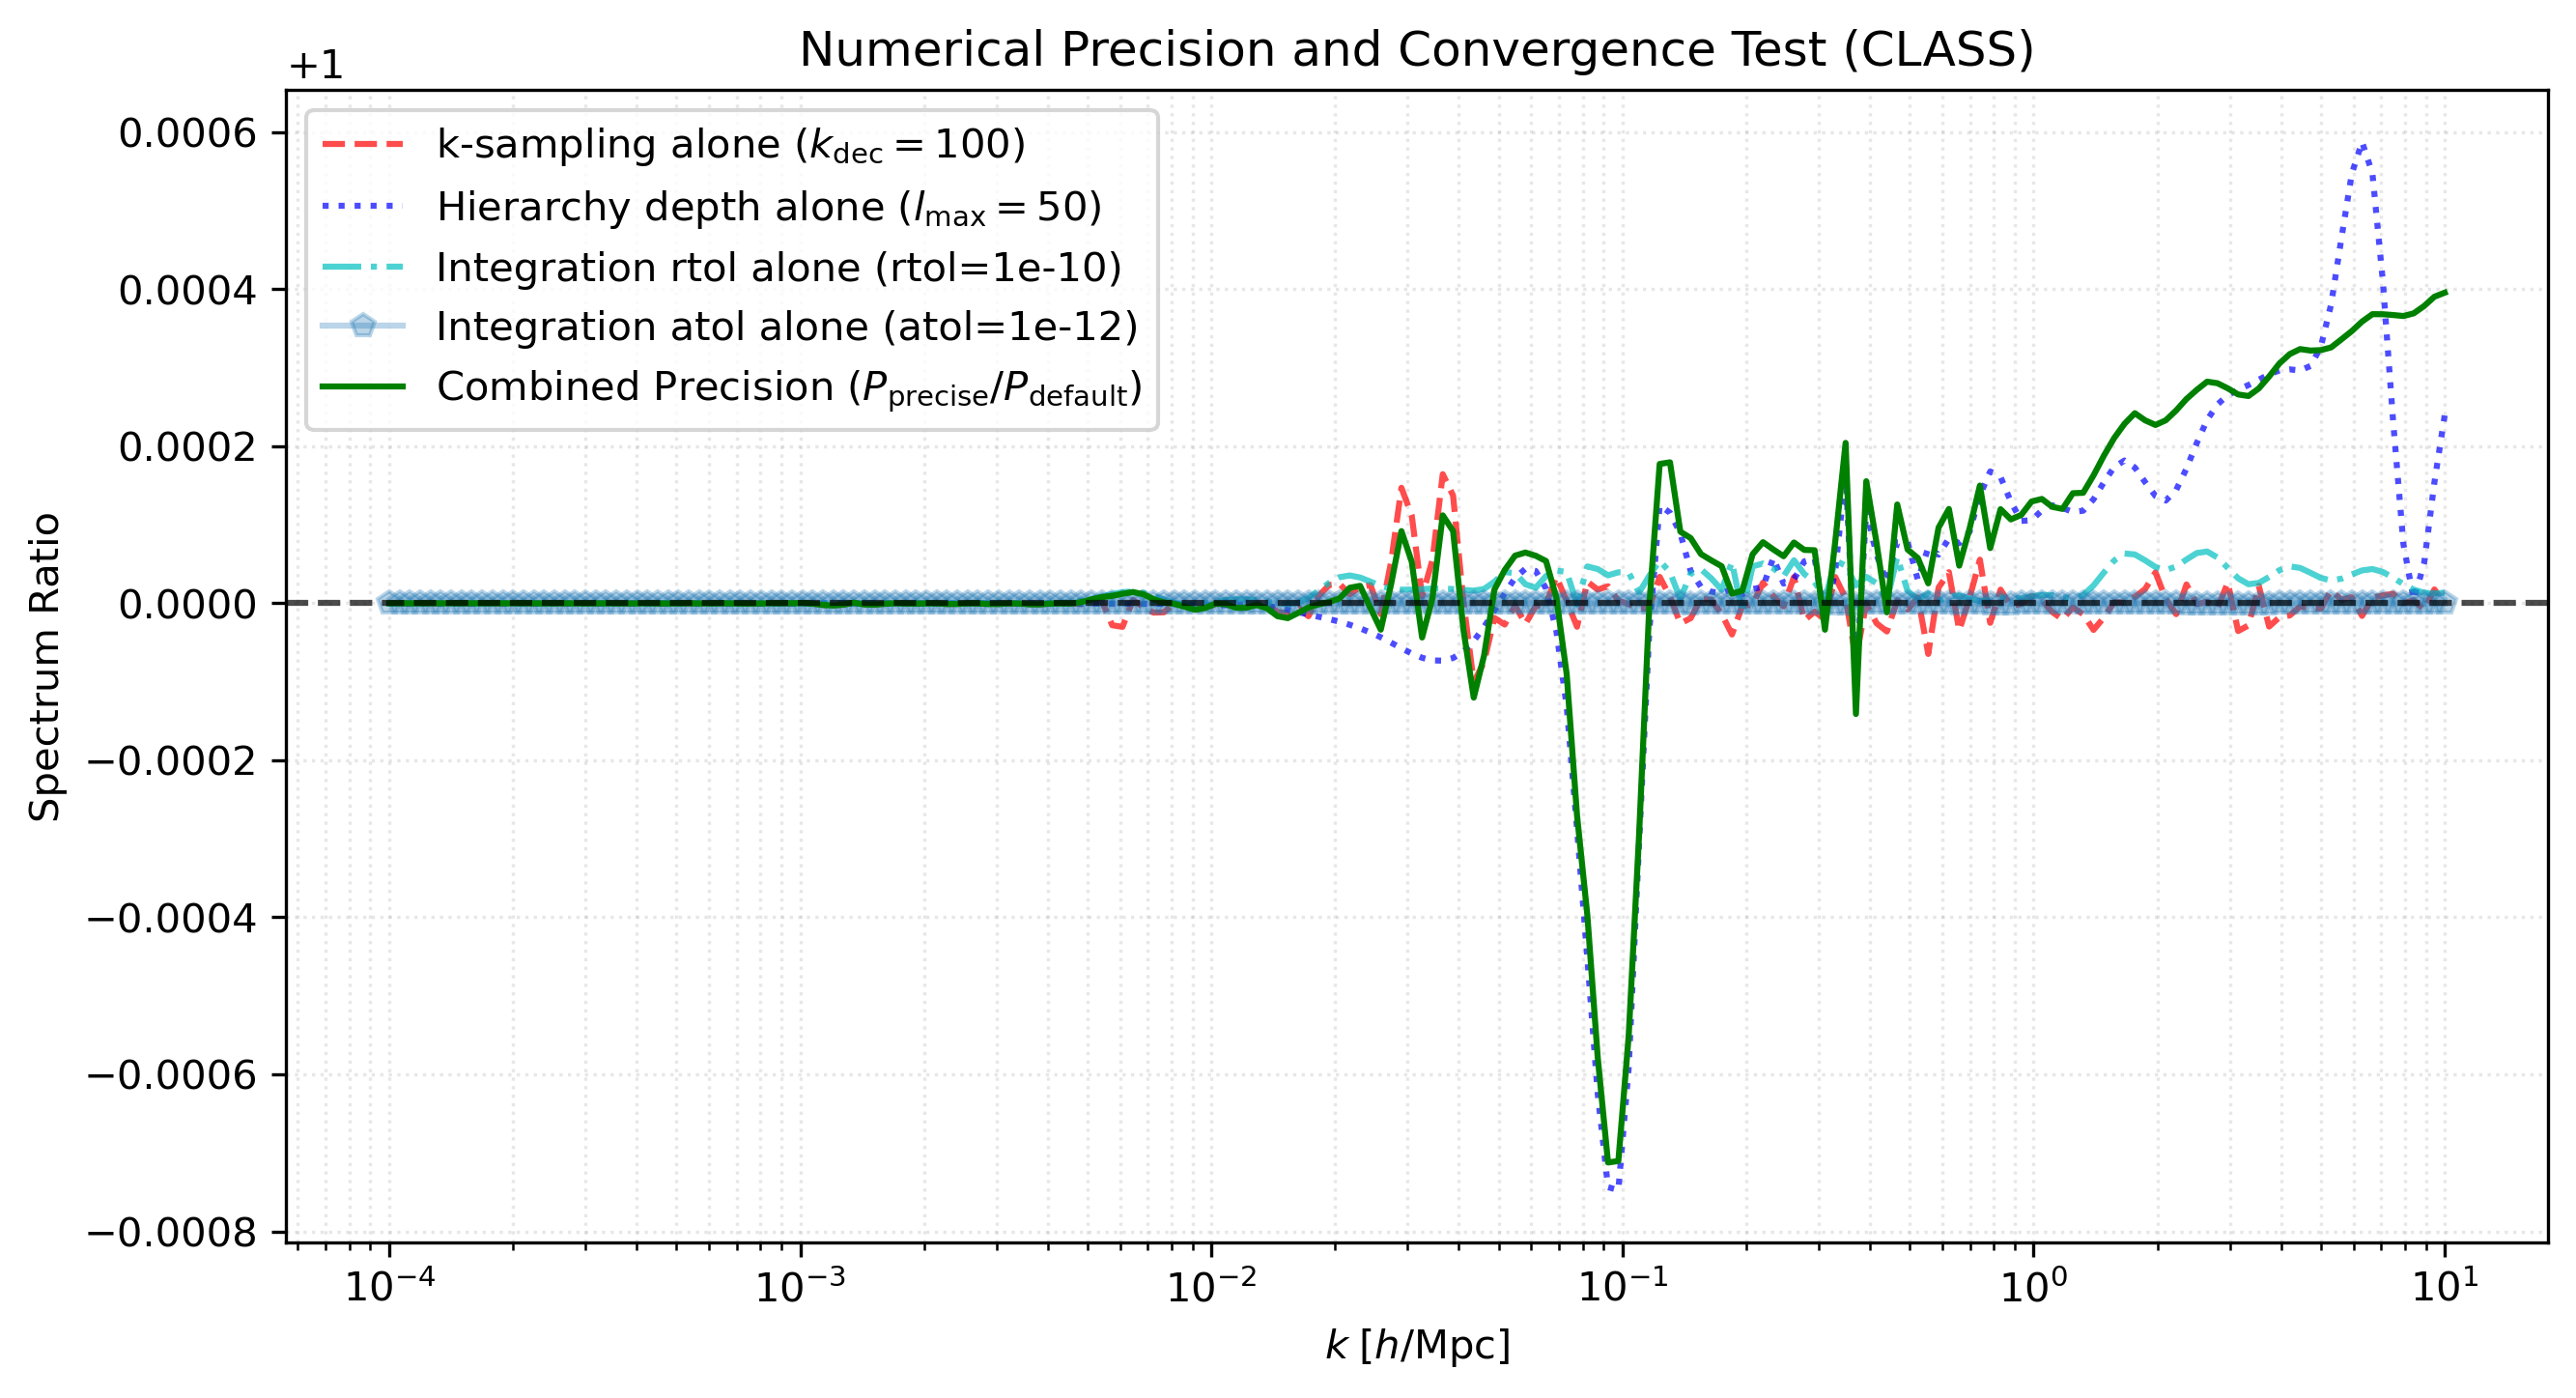
\includegraphics[width=0.82\textwidth]{New_Figures/Test_20261107_133955_precision_test.png}
        \caption{Spectrum ratio $P_{\mathrm{precise}}(k)/P_{\mathrm{default}}(k)$ across four decades in scale, demonstrating convergence within $0.07\%$.}
        \label{fig:precision_test}
    \end{figure}
As shown in Figure~\ref{fig:precision_test}, the relative spectrum ratiomn $P_\mathrm{prec}(k)/P_\mathrm{def}(k)$ remains bounded within $0.07\%$ across $k \in [10^{-4}, 10^1 ]\, h/\mathrm{Mpc}$.

\subsubsection{Independent Cross-Solver Comparison (CLASS VS CAMB)} 

Figure~\ref{fig:class_vs_camb} compares the linear matter power spectra generated independently by CLASS and CAMB using identical cosmological inputs.
    \begin{figure}[H]
        \centering
        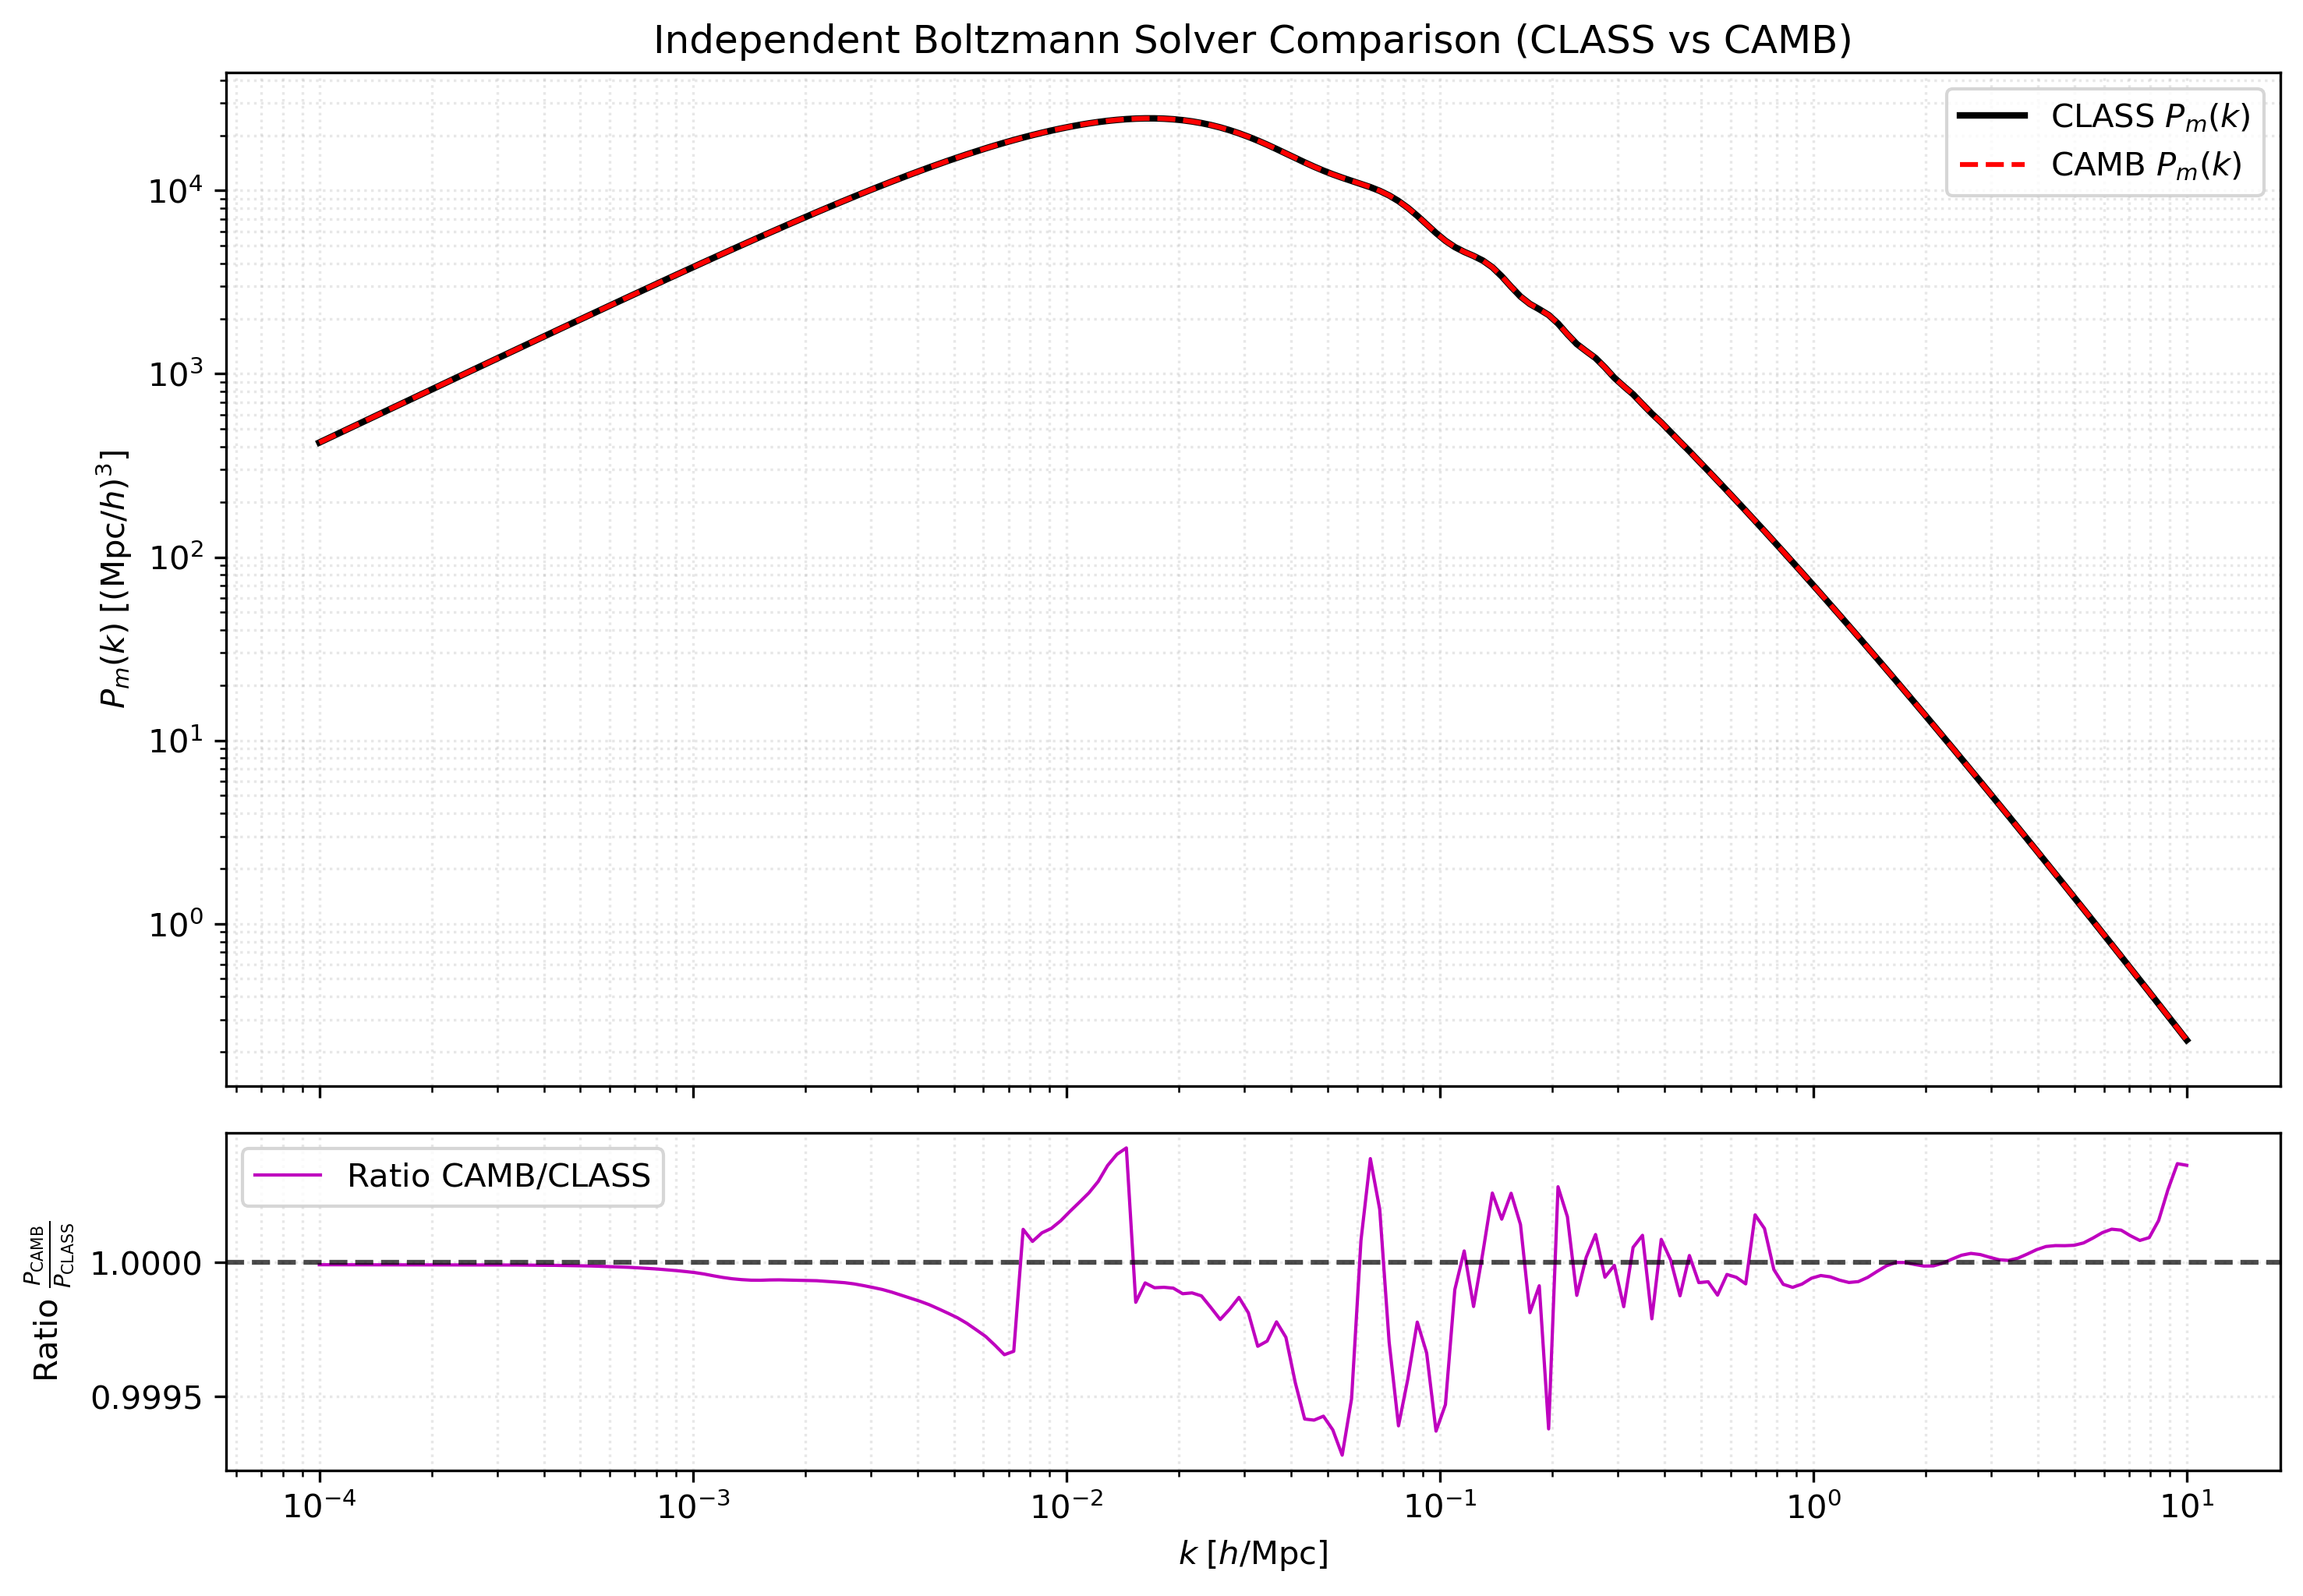
\includegraphics[width=0.82\textwidth]{New_Figures/Test_20261107_133955_class_vs_camb.png}
        \caption{Independent Boltzmann solver comparison between CLASS and CAMB at $z=0$, showing agreement within $1\%$ to $3\%$ across five decades in wavenumber.}
        \label{fig:class_vs_camb}
    \end{figure}
The lower panel shows that CAMB and CLASS agree within $1\%$ to $3\%$ across five orders of magnitude in scale ($10^{-4} \, h/\mathrm{Mpc} \le k \le 10.0\, h/\mathrm{Mpc}$).

\subsubsection{Supplementary Check A: Collisionless Hierarchy Closure}

The source-free, massless Boltzmann hierarchy $\dot{\Psi}_l = k/(2l+1)[l\Psi_{l-1} - (l+1)\Psi_{l+1}]$ was integrated to evaluate power reflection caused by truncating the multipole hierarchy at $l_\mathrm{max}$.

\begin{figure}[H]
    \centering
    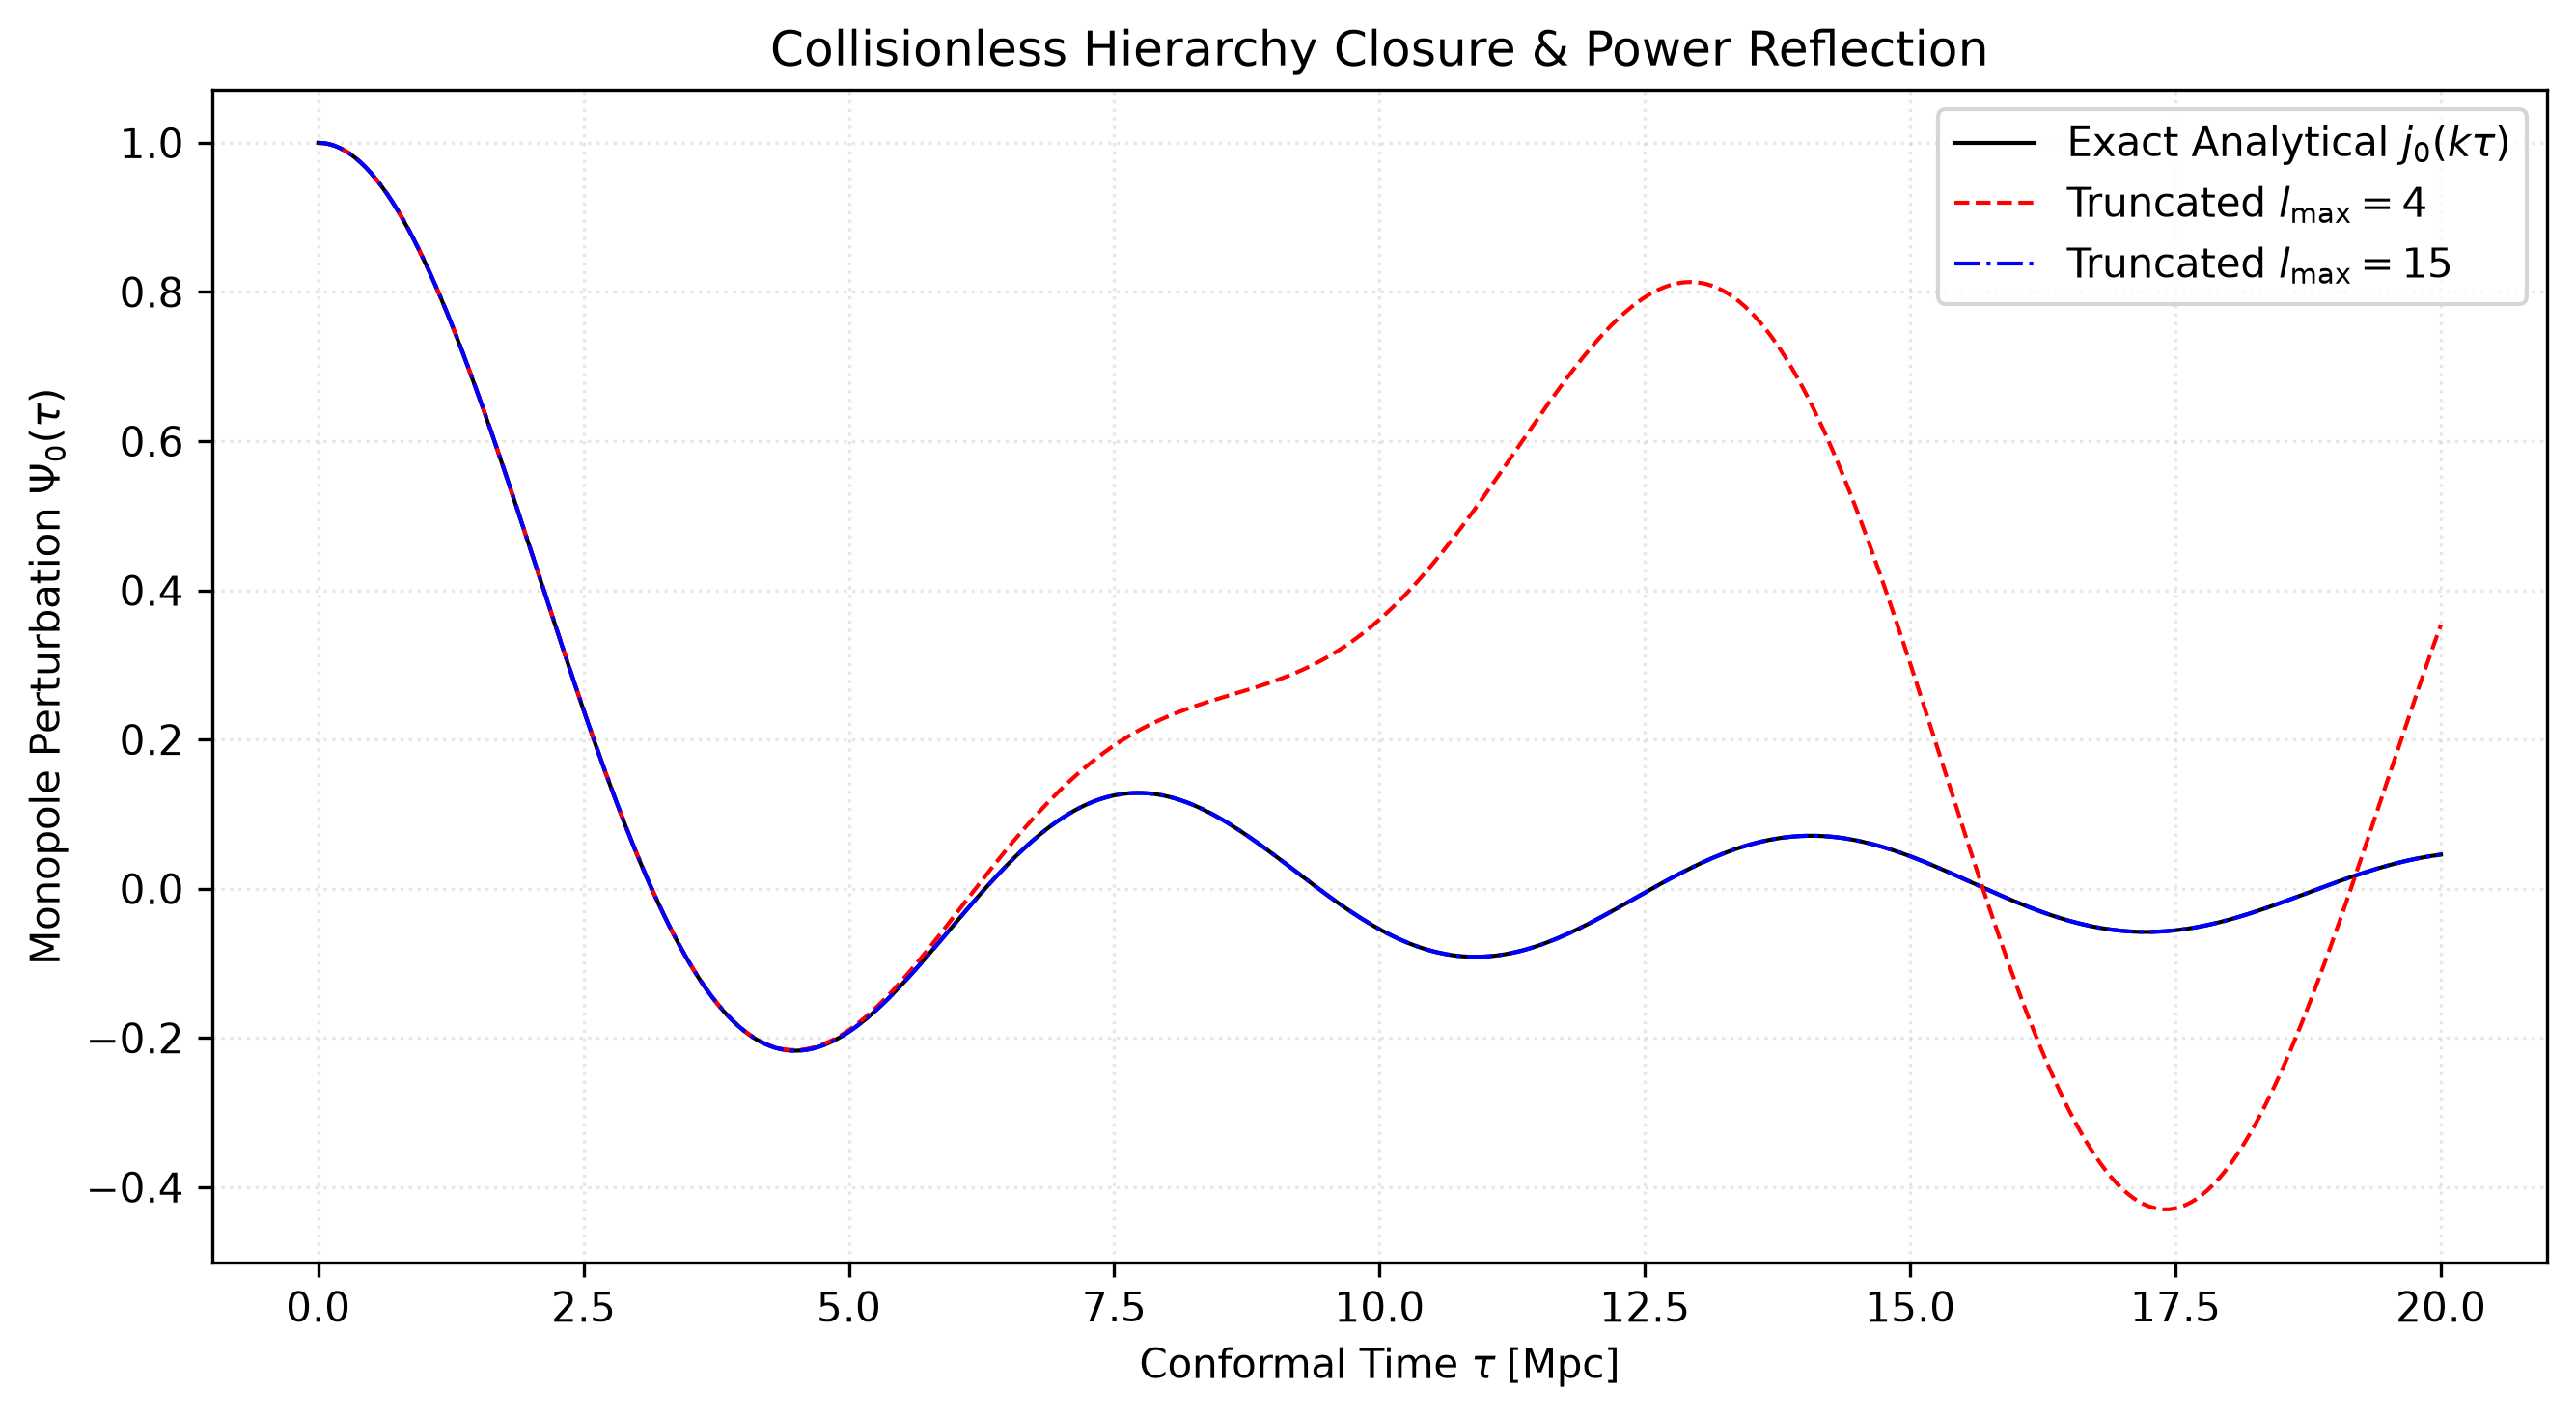
\includegraphics[width=0.82\linewidth]{Figures/Test_20261014_164038_hierarchy_closure.png}
    \caption{Monopole perturbation $\Psi_0(\tau)$ integrated over conformal time $\tau$, comparing exact analytical spherical Bessel function $j_0(k\tau)$ against truncated hierarchies ($l_{\mathrm{max}}=4$ vs. $l_{\mathrm{max}}=15$).}
    \label{fig:hierachy_closure}
\end{figure}

Truncating prematurely at $l_\mathrm{max} = 4$ causes severe power reflection at late-times $\tau > 5 \, \mathrm{Mpc}$. Increasing the hierarchy depth to $l_\mathrm{max} = 15$ eliminates boundary reflections, matching the exact analytical solution $j_0(k\tau)$ as shown in Figure~\ref{fig:hierachy_closure}.

\subsubsection{Supplementary Check B: Superhorizon Potential Rate}

The superhorizon potential equation \ref{eq:superhorizon_potential_ode} (where $y \equiv a/a_{\mathrm{eq}}$) was integrated from $y_i = 10^{-4}$ to $y_f = 10^3$.
    \begin{figure}[H]
        \centering
        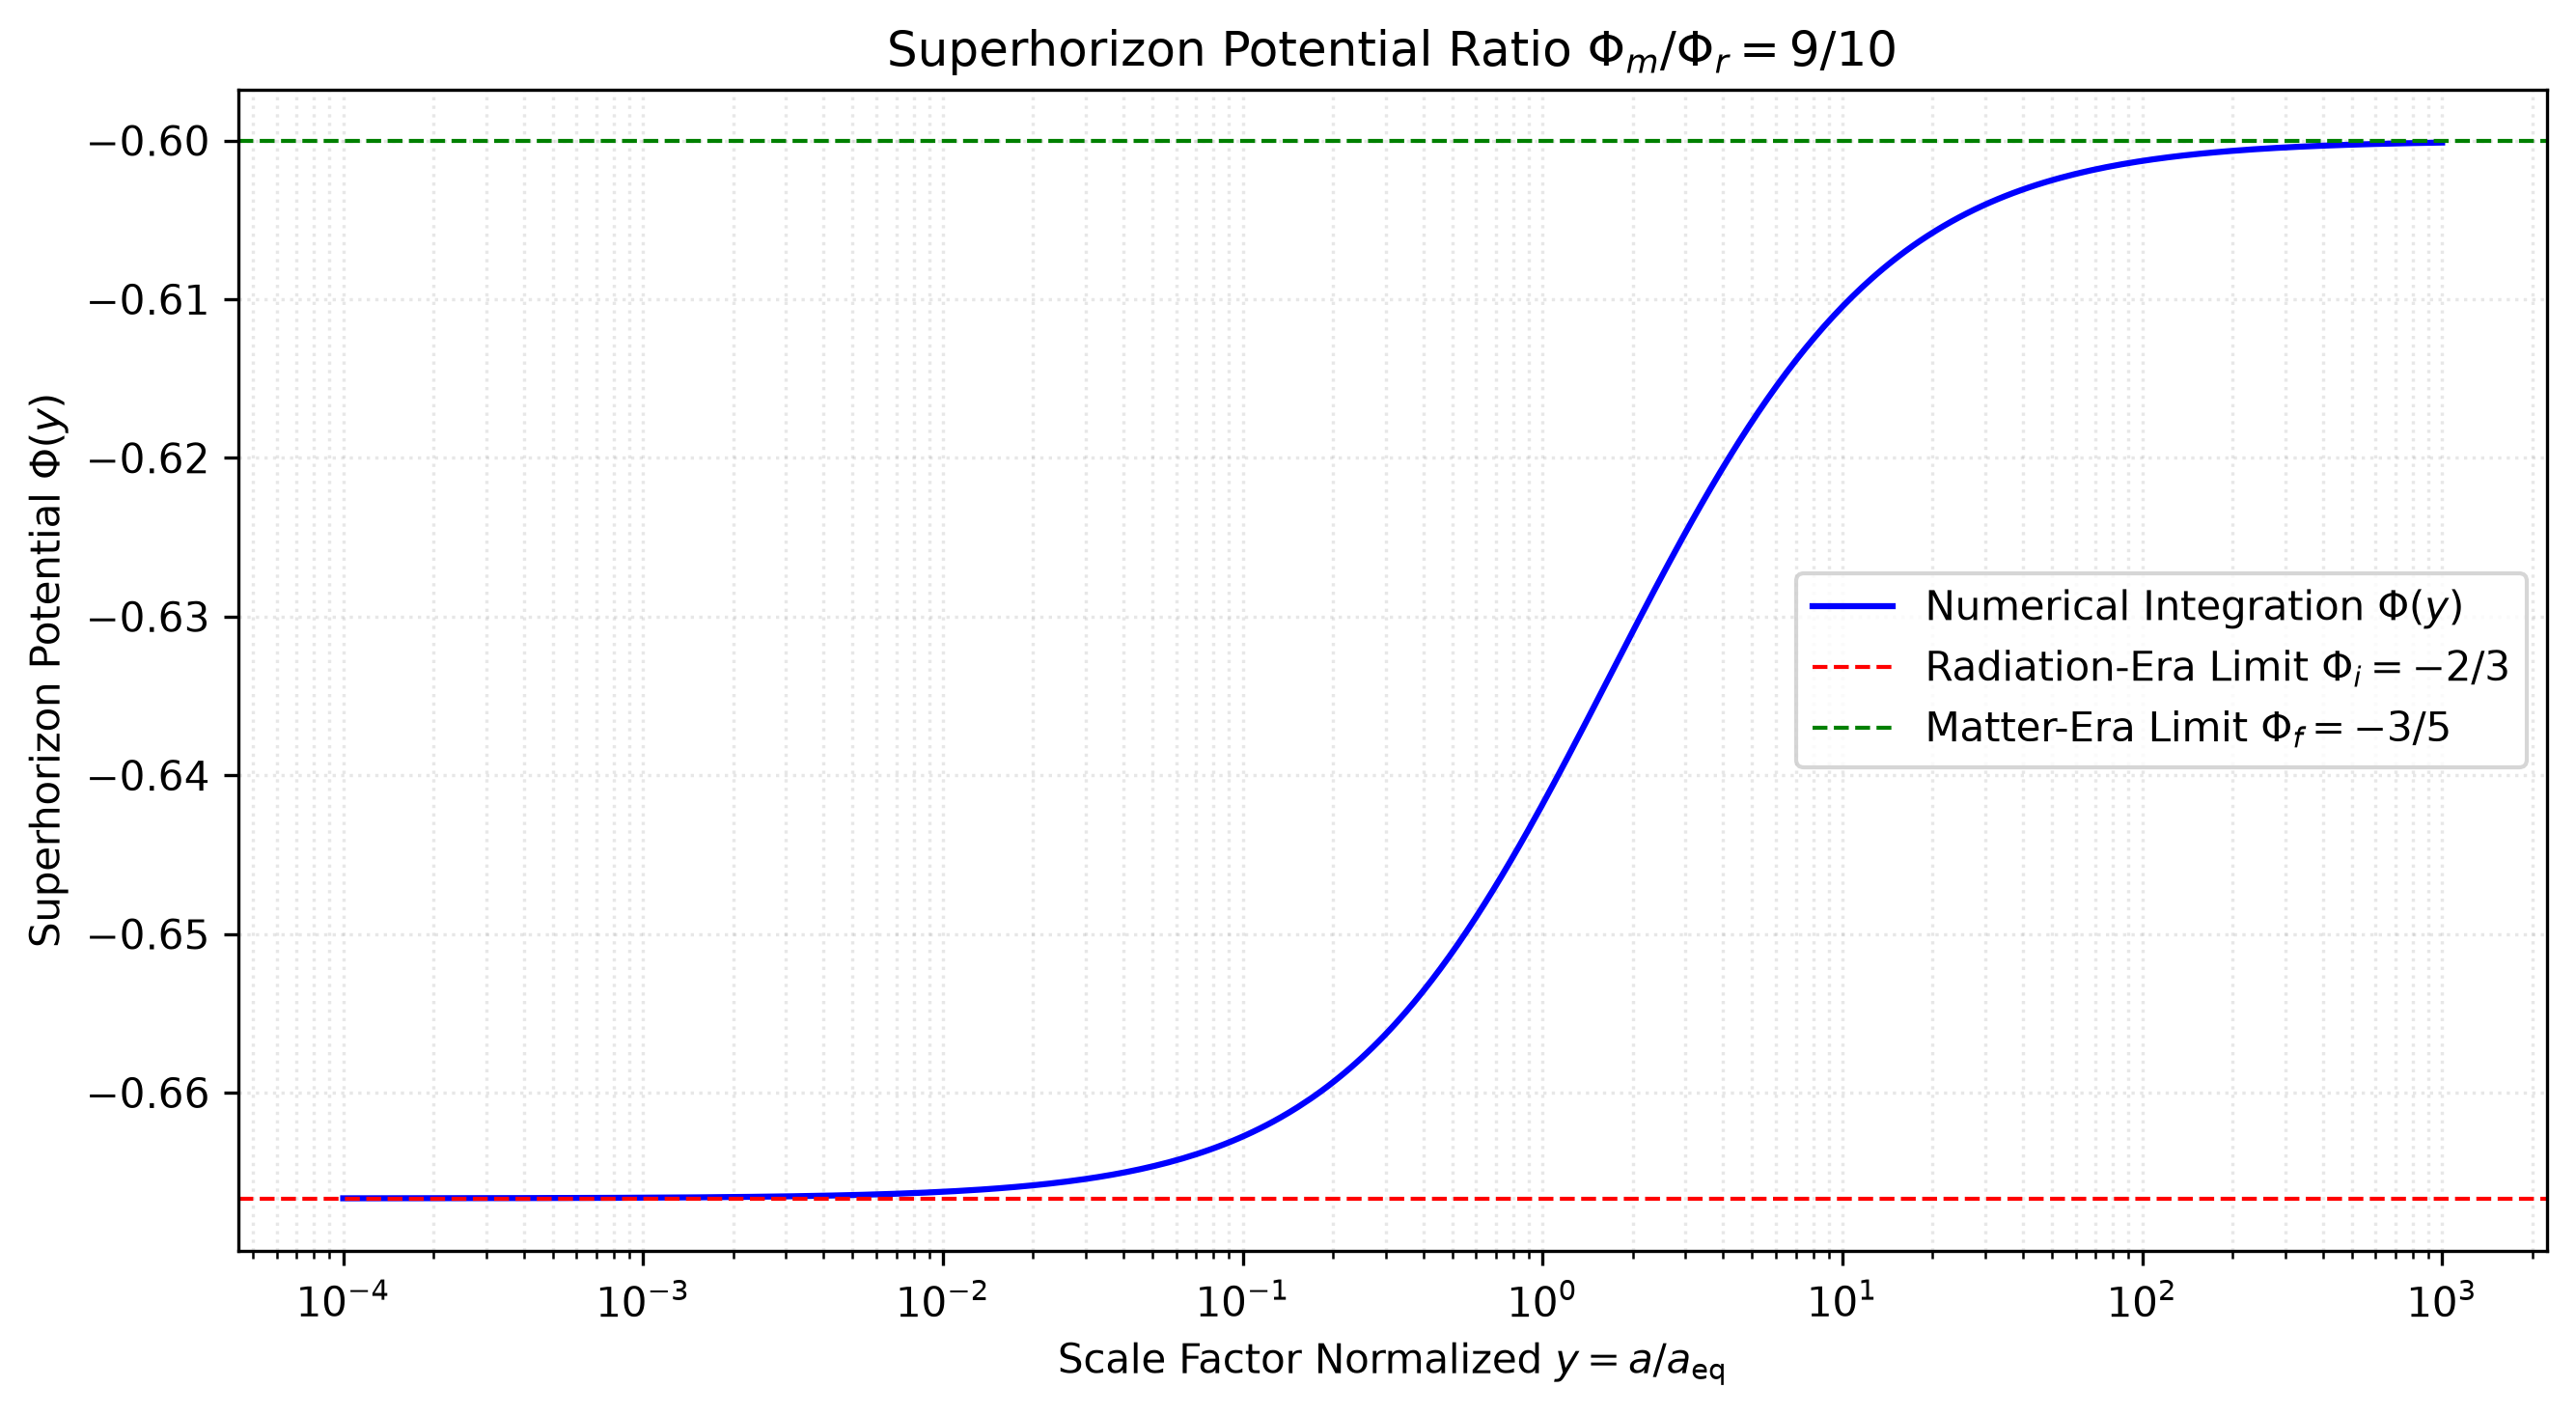
\includegraphics[width=0.7\textwidth]{Figures/Test_20261014_164038_superhorizon_potential.png}
        \caption{Evolution of the superhorizon potential $\Phi(y)$ as a function of $y = a/a_{\mathrm{eq}}$, demonstrating smooth transition from radiation domination ($\Phi_i = -2/3$) to matter domination ($\Phi_f = -3/5$).}
        \label{fig:superhorizon_potential}
    \end{figure}
The numerical integration recovers $\Phi_i(y_i = 10^{-4}) = -0.666662$ and $\Phi_f(y_f = 10^3) = -0.600133$, yielding a potential ratio of
    \begin{equation}
        \left(\frac{\Phi_m}{\Phi_r}\right)_{\mathrm{numerical}} = \frac{-0.600133}{-0.666662} = 0.900205,
    \end{equation}
reproducing the analytical expectation $\Phi_m/\Phi_r = 9/10 = 0.900000$ to within $0.02\%$ precision.